\section{$\PTIME^{\NP}$-hardness of MC for $\AB$ and $\AbarE$}\label{sec:ABhard}

In this section, we show that the $\PTIME^{\NP}$-complete problem named \emph{Sequentially Nested SATisfiability} (SNSAT~\cite{LMS01}) can be reduced to MC for formulas of the fragment $\AB$ (and similarly $\AbarE$), thus proving $\PTIME^{\NP}$-hardness of the latter.
%
%we prove that model checking for $\AB$ (and $\AbarE$) formulas is hard for the class $\PTIME^{\NP}$ by reducing the $\PTIME^{\NP}$-complete problem SNSAT to it; 
SNSAT 
%(the abbreviation of Sequentially Nested SATisfiability) 
is a logical problem featuring a series of nested satisfiability questions.
%We start by introducing SNSAT.

\begin{definition}\label{snsat}
An instance $\mathcal{I}$ of SNSAT consists of 
%\begin{itemize}
%    \item 
    a set of $n$ Boolean variables $X=\{x_1,\ldots ,x_n\}$ and
 %   \item 
   a set of $n$ Boolean formulas 
\[\{F_1(Z_1), F_2(x_1,Z_2),\ldots , F_n(x_1,\ldots , x_{n-1}, Z_n)\}, \] where, for $i=1,\ldots , n$, $F_i(x_1, \ldots ,x_{i-1},Z_i)$ has variables in $\{x_1, \ldots ,x_{i-1}\}$ and in the set of private variables $Z_i=\{z_i^1,\ldots ,z_i^{j_i}\}$, 
%the latter being a set of variables
%
%\emph{local to $F_i$}, that is,
% 
that is, $Z_i\cap Z_t=\emptyset$, for $t \neq i$, and $X\cap Z_i=\emptyset$.
%\end{itemize}
We denote by $|\mathcal{I}|$ the cardinality $|X| =n$.

Let $v_\mathcal{I}$ be a truth-assignment of the variables in $X$ defined as follows: 
\[
    v_\mathcal{I}(x_i)=\top \iff
    \begin{array}{l}
        F_i(v_\mathcal{I}(x_1), \ldots, v_\mathcal{I}(x_{i-1}), Z_i)\text{ is satisfiable} 
        %\\
  %      \text{(by assigning suitable values to the local variables $z_i^1,\ldots ,z_i^{j_i}\in Z_i$).} 
    \end{array}
\]
(by a suitable truth-assignment  to the private
variables $z_i^1,\ldots ,z_i^{j_i}\in Z_i$).  
 
SNSAT is the problem of deciding, given an instance $\mathcal{I}$ with $|\mathcal{I}|=n$, whether
$v_\mathcal{I}(x_n)=\top$ or not. In such a case, we say that $\mathcal{I}$ is a positive instance of SNSAT.
\end{definition}

Given an SNSAT instance $\mathcal{I}$, with $|\mathcal{I}|=n$, the truth-assignment $v_\mathcal{I}$ is unique and it can be easily computed by a $\PTIME^{\NP}$ algorithm as follows. A first query to a SAT oracle determines whether $v_\mathcal{I}(x_1)$ is $\top$ or $\bot$, since $v_\mathcal{I}(x_1)=\top$ if and only if $F_1(Z_1)$ is satisfiable. Then, we replace $x_1$ by the value $v_\mathcal{I}(x_1)$ in $F_2(x_1,Z_2)$ and another query to the SAT oracle is performed to determine whether $F_2(v_\mathcal{I}(x_1),Z_2)$ is satisfiable, yielding the value of $v_\mathcal{I}(x_2)$. This step is iterated other $n-2$ times, finally obtaining the value of $v_\mathcal{I}(x_n)$. 

Let $\mathcal{I}$ be an instance of SNSAT, with $|\mathcal{I}|=n$. We now show how to build a finite Kripke structure $\Ku_\mathcal{I}$ and an $\AB$ formula $\Phi_\mathcal{I}$ in polynomial time, such that $\mathcal{I}$ is a positive instance of SNSAT if and only if $\Ku_\mathcal{I}\models \Phi_\mathcal{I}$. Such a reduction is inspired by similar constructions from~\cite{LMS01}.

Let $Z=\bigcup_{i=1}^n Z_i$ and let $\tilde{R}=\{r_i \mid i=1,\ldots , n\}$ and $\tilde{R}_i=\tilde{R}\setminus \{r_i\}$ be $n+1$ sets of auxiliary variables.
The Kripke structure $\Ku_\mathcal{I}$ consists of a suitable composition of $n$ instances of a \emph{gadget} (an instance  for each variable $x_1,\ldots , x_n\in X$). The structure of the gadget for $x_i$, with $1\leq i\leq n$, is shown in Figure~\ref{gadget}, assuming that the labeling of states (nodes) is defined as follows:
\begin{itemize}
	\item $\Lab(w_{x_i})=X \cup Z \cup \{s,t\} \cup \tilde{R}_i$, and
	%\\
    	$\Lab(\overline{w_{x_i}})=(X\setminus \{x_i\}) \cup Z \cup \{s,t\} \cup \tilde{R}_i \cup \{p_{\overline{x_i}}\}$;
	\item for $u_i=1,\ldots , j_i$, $\Lab(w_{z_i^{u_i}})=X \cup Z \cup \{s,t\} \cup \tilde{R}_i$, and\\
	    $\Lab(\overline{w_{z_i^{u_i}}})=X \cup (Z\setminus \{z_i^{u_i}\}) \cup \{s,t\} \cup \tilde{R}_i$;
	\item $\Lab(\overline{s_i})=X \cup Z \cup \{t\} \cup \tilde{R}_i$.
\end{itemize}

\begin{figure}[p]
  \centering
  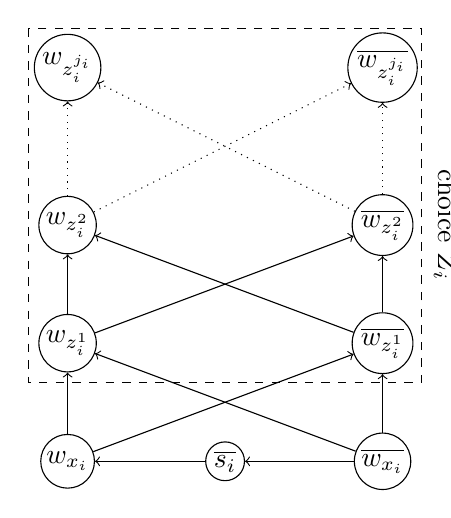
\begin{tikzpicture}[every node/.style={circle, draw, inner sep=1pt}]

\node (v3) at (-2,0.5) {$w_{x_i}$};
\node (v2) at (0,0.5) {$\overline{s_i}$};
\node (v1) at (2,0.5) {$\overline{w_{x_i}}$};
\draw [->] (v1) edge (v2);
\draw [->] (v2) edge (v3);
\draw [dashed] (-2.5,6) rectangle (2.5,1.5);

\draw [use as bounding box,draw=none] (-2.5,6) rectangle (2.5,0.2);

\node (v4) at (-2,2) {$w_{z_i^1}$};
\node (v6) at (2,2) {$\overline{w_{z_i^1}}$};
\node (v5) at (-2,3.5) {$w_{z_i^2}$};
\node (v7) at (2,3.5) {$\overline{w_{z_i^2}}$};
\node (v8) at (-2,5.5) {$w_{z_i^{j_i}}$};
\node (v9) at (2,5.5) {$\overline{w_{z_i^{j_i}}}$};
\draw [->] (v4) edge (v5);
\draw [->] (v6) edge (v7);
\draw [->] (v4) edge (v7);
\draw [->] (v6) edge (v5);

\draw [->,dotted] (v5) edge (v8);
\draw [->,dotted] (v7) edge (v9);
\draw [->,dotted] (v7) edge (v8);
\draw [->,dotted] (v5) edge (v9);
\draw [->] (v3) edge (v4);
\draw [->] (v3) edge (v6);
\draw [->] (v1) edge (v4);
\draw [->] (v1) edge (v6);

\node [draw=none,rotate=-90] (ch) at (2.8,3.5) {choice $Z_i$};
\end{tikzpicture}
  \caption{The gadget for $x_i$.}\label{gadget}
\end{figure}

\begin{figure}[p]
  \rotatebox{-90}{\resizebox{!}{\linewidth}{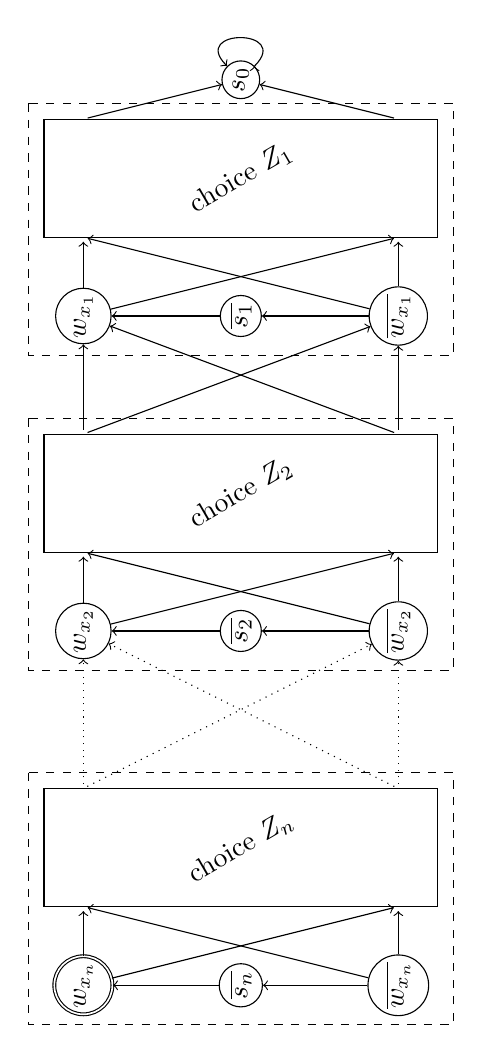
\begin{tikzpicture}[every node/.style={circle, draw, inner sep=1pt}]

\node [rotate=90] (v3) at (-2,0.5) {$w_{x_1}$};
\node [rotate=90] (v2) at (0,0.5) {$\overline{s_1}$};
\node [rotate=90] (v1) at (2,0.5) {$\overline{w_{x_1}}$};
\draw [->] (v1) edge (v2);
\draw [->] (v2) edge (v3);
\draw  (-2.5,3) rectangle (2.5,1.5) node[midway,draw=none,rotate=30] {choice $Z_1$};;

\node [draw=none] (v4) at (-2,1.5) {};
\node [draw=none] (v6) at (2,1.5) {};

\draw [->] (v3) edge (v4);
\draw [->] (v1) edge (v6);


%%%%%
\node [double,rotate=90]  (v13) at (-2,-8) {$w_{x_n}$};
\node [rotate=90] (v12) at (0,-8) {$\overline{s_n}$};
\node [rotate=90] (v11) at (2,-8) {$\overline{w_{x_n}}$};
\draw [->] (v11) edge (v12);
\draw [->] (v12) edge (v13);
\draw  (-2.5,-5.5) rectangle (2.5,-7) node[midway,draw=none,rotate=30] {choice $Z_n$};;

\node [draw=none] (v14) at (-2,-7) {};
\node [draw=none] (v16) at (2,-7) {};

\draw [->] (v13) edge (v14);
\draw [->] (v11) edge (v16);



%%%%
\node [rotate=90] (v23) at (-2,-3.5) {$w_{x_2}$};
\node [rotate=90] (v22) at (0,-3.5) {$\overline{s_2}$};
\node [rotate=90] (v21) at (2,-3.5) {$\overline{w_{x_2}}$};
\draw [->] (v21) edge (v22);
\draw [->] (v22) edge (v23);
\draw  (-2.5,-1) rectangle (2.5,-2.5) node[midway,draw=none,rotate=30] {choice $Z_2$};;

\node [draw=none] (v24) at (-2,-2.5) {};
\node [draw=none] (v26) at (2,-2.5) {};

\draw [->] (v23) edge (v24);
\draw [->] (v21) edge (v26);





\node [draw=none] (v8) at (-2,-5.5) {};
\node [draw=none] (v18) at (2,-5.5) {};
\node [draw=none] (v29) at (2,-1) {};
\node [draw=none] (v19) at (-2,-1) {};
\draw [->, dotted] (v8) edge (v23);
\draw [->, dotted] (v18) edge (v21);
\draw [->] (v19) edge (v3);
\draw [->] (v29) edge (v1);

\node [rotate=90] (v9) at (0,3.5) {$s_0$};
\node [draw=none] (v30) at (-2,3) {};
\draw [->,looseness=5] (v9.south east) edge (v9.north east);

\node [draw=none] (v10) at (2,3) {};

\draw [->] (v19) edge (v1);
\draw [->] (v29) edge (v3);
\draw [->,dotted] (v18) edge (v23);
\draw [->,dotted] (v8) edge (v21);
\draw [->] (v30) edge (v9);
\draw [->] (v10) edge (v9);
\draw [->] (v13) edge (v16);
\draw [->] (v11) edge (v14);
\draw [->] (v23) edge (v26);
\draw [->] (v21) edge (v24);
\draw [->] (v3) edge (v6);
\draw [->] (v1) edge (v4);

\draw [dashed] (-2.7,3.2) rectangle (2.7,0);
\draw [dashed] (-2.7,-0.8) rectangle (2.7,-4);
\draw [dashed] (-2.7,-5.3) rectangle (2.7,-8.5);

%%%%%%%%%
%\node [double] (v33) at (-2,-9) {$y$};
%\draw [->] (v33) edge (v13);
\end{tikzpicture}}}
  \caption{Kripke structure $\Ku_\mathcal{I}$ associated with an SNSAT instance $\mathcal{I}$, with $|\mathcal{I}|=n$. Note that the states $\overline{s_n}$ and $\overline{w_{x_n}}$ are unreachable.}\label{fullKripke}
\end{figure}

The Kripke structure  $\Ku_\mathcal{I}$ is obtained by sequentializing (adding suitable edges) the $n$ instances of the gadget (in reverse order, from $x_n$ to $x_1$), adding a collector terminal state $s_0$, with labeling $\Lab(s_0)=X \cup Z \cup \{s\} \cup \tilde{R}$, and setting $w_{x_n}$ as the initial state. The overall construction is reported in Figure~\ref{fullKripke}. Formally, we have \[\Ku_\mathcal{I}=(\Prop, \States,\Edges,\Lab,w_{x_n}),\] 
where, in particular, $\Prop=X \cup Z \cup \{s,t\} \cup \tilde{R}\cup\{p_{\overline{x_i}}\mid i=1,\ldots ,n\}$ and \[\States=\{s_0\}\cup\bigcup_{i=1}^n\big(\{\overline{s_i},w_{x_i},\overline{w_{x_i}}\}\cup\{w_{z_i^{u_i}},\overline{w_{z_i^{u_i}}}\mid u_i=1,\ldots,j_i\}\big).\]
%
The Kripke structure $\Ku_\mathcal{I}$ features the following properties:
\begin{itemize}
	\item any trace satisfying $s$ does not pass through any $\overline{s_i}$, for $1\leq i\leq n$;
	\item any trace \emph{not} satisfying $t$ has $s_0$ as its last state;
	\item any trace \emph{not} satisfying $r_i$ passes through some state of the $i$-th gadget, for $1\leq i\leq n$;
	\item the only trace satisfying $p_{\overline{x_i}}$ is $\overline{w_{x_i}}$ (note that $|\overline{w_{x_i}}|=1$), for $1\leq i\leq n$.
\end{itemize}

A trace $\rho\in\Trk_{\Ku_\mathcal{I}}$ \emph{induces} a truth assignment of all the proposition letters, denoted by $\omega_\rho$, which is defined as $\omega_\rho(y)=\top \iff \Ku_\mathcal{I},\rho\models y$, for any letter $y$. 
In the following, we shall write $\omega_\rho(Z_i)$ for $\omega_\rho(z_i^1),\ldots , \omega_\rho(z_i^{j_i})$.
In particular, if $\rho$ starts from some state $w_{x_i}$ or $\overline{w_{x_i}}$, and satisfies $s\wedge \neg t$ (that is, it reaches the collector state $s_0$ without visiting any node $\overline{s_j}$, for $1\leq j \leq i$), $\omega_\rho$ fulfills the following conditions: 
for $1\leq m\leq i$,
\begin{itemize}
	\item if $w_{x_m}\!\in\!\states(\rho)$, then $\omega_\rho(x_m)\!=\!\top$, and if $\overline{w_{x_m}}\!\in\!\states(\rho)$, then $\omega_\rho(x_m)\!=\!\bot$;
	\item for $1\leq u_m\leq j_m$, if $w_{z_m^{u_m}}\in\states(\rho)$, then $\omega_\rho(z_m^{u_m})=\top$, and if $\overline{w_{z_m^{u_m}}}\in\states(\rho)$, then $\omega_\rho(z_m^{u_m})=\bot$.
\end{itemize}	
It easily follows that $\Ku_\mathcal{I},\rho\models F_m(x_1,\ldots , x_{m-1}, Z_m)$ if and only if 
$F_m(\omega_\rho(x_1), \ldots ,\allowbreak \omega_\rho(x_{m-1}),\omega_\rho(Z_m)) = \top$.
%
%
Finally, let $\mathcal{F}_\mathcal{I}=\{\psi_k \mid 0\leq k\leq n+1\}$ be the set of formulas defined as: 
\[\psi_0=\bot \mbox{ and, for  }k\geq 1,\]
%
\begin{equation*}
\psi_k = \hsA \underbrace{\left[\begin{array}{c}
(s\wedge \neg t) \wedge \displaystyle{\bigwedge_{i=1}^n} \Big((x_i\wedge \neg r_i)\rightarrow F_i(x_1, \ldots, x_{i-1}, Z_i)\Big) \\ 
\wedge \\ 
\hsBu \Big( \Big(\displaystyle{\bigvee_{i=1}^n} \hsA p_{\overline{x_i}}\Big)\rightarrow \hsA\big(\neg s \wedge \Length_2\wedge \hsA (\Length_2\wedge \neg\psi_{k-1})\big)\Big)
\end{array}\right]}_{\text{\normalsize $\varphi_k$}} ,
\end{equation*}
where $\Length_2=\hsB \top \wedge \hsBu\hsBu\bot$ (Example~\ref{example:length}) is satisfied only by traces of length 2.
The first conjunct of $\varphi_k$, i.e, $s\wedge \neg t$, forces the trace to reach the collector state $s_0$, without visiting any state $\overline{s_j}$. The second conjunct checks that if the trace assigns the truth value $\top$ to $x_m$ passing through $w_{x_m}$, with $1\leq m \leq n$, then $F_m(x_1,\ldots,x_{m-1},Z_m)$ is satisfied by $\omega_\rho$ (which amounts to say that the SAT problem connected with $Z_m$ has a positive answer, for the selected values of $x_1,\ldots,x_{m-1}$).
Conversely, the third conjunct ensures that if the trace assigns the truth value $\bot$ to some $x_m$ by passing through $\overline{w_{x_m}}$, then, intuitively, the SAT problem connected with $Z_m$ has no assignment satisfying $F_m(x_1, \ldots, x_{m-1}, Z_m)$. As a matter of fact, if $\rho$ satisfies $\varphi_k$, for some $k\geq 2$, and assigns $\bot$ to $x_m$, then there is a prefix $\tilde{\rho}$ of $\rho$ ending in $\overline{w_{x_m}}$. Since  $\bigvee_{i=1}^n\hsA p_{\overline{x_i}}$ is satisfied by $\tilde{\rho}$, $\hsA\big(\neg s \wedge \Length_2\wedge \hsA (\Length_2\wedge \neg\psi_{k-1})\big)$ must be satisfied as well. The only possibility is that the trace $\overline{s_m}\cdot w_{x_m}$ does not model $\psi_{k-1}$, as $\overline{w_{x_m}}\cdot \overline{s_m}$ has to model $\hsA (\Length_2\wedge \neg\psi_{k-1})$. However, since $\psi_{k-1}=\hsA\varphi_{k-1}$, this holds if and only if $\Ku, w_{x_m}\not \models\psi_{k-1}$.

The following theorem states the correctness of the construction. Its proof can be found in Appendix~\ref{proof:thcorr}.
\begin{theorem}\label{thcorr} 
Let $\mathcal{I}$ be an instance of SNSAT, with $|\mathcal{I}|=n$, and let $\Ku_\mathcal{I}$ and $\mathcal{F}_\mathcal{I}$
%$=\{\psi_k \mid 0\leq k\leq n+1\}$ 
be defined as above. For all $0\leq k\leq n+1$ and all $r=1,\ldots , n$, it holds that:
	\begin{enumerate}
		\item if $k\geq r$, then $v_\mathcal{I}(x_r)=\top \iff \Ku_\mathcal{I},w_{x_r}\models \psi_k;$
		%\[v_\mathcal{I}(x_r)=\top \iff \Ku_\mathcal{I},w_{x_r}\models \psi_k;\]
		\item if $k\geq r+1$, then $v_\mathcal{I}(x_r)=\bot \iff \Ku_\mathcal{I},\overline{w_{x_r}}\models \psi_k.$
		%\[v_\mathcal{I}(x_r)=\bot \iff \Ku_\mathcal{I},\overline{w_{x_r}}\models \psi_k.\]
	\end{enumerate}
\end{theorem}

The correctness of the reduction from SNSAT to MC for $\AB$ follows.

\begin{corollary}\label{corol:c} Let $\mathcal{I}$ be an instance of SNSAT, with $|\mathcal{I}|=n$, and let $\Ku_\mathcal{I}$ and $\mathcal{F}_\mathcal{I}$
%=\{\psi_k \mid 0\leq k\leq n+1\}$ 
be defined as above. Then, 
$v_\mathcal{I}(x_n)=\top \iff \Ku_\mathcal{I}\models \hsBu\bot \rightarrow\psi_n$.
\end{corollary}
\begin{proof}
By Theorem~\ref{thcorr}, $v_\mathcal{I}(x_n)=\top \iff \Ku_\mathcal{I},w_{x_n}\models \psi_n$. If $v_\mathcal{I}(x_n)=\top$ then $\Ku_\mathcal{I},w_{x_n}\models \psi_n$ and, since $w_{x_n}$ is the only initial trace satisfying $\hsBu\bot$ (this formula is satisfied by traces having length equal to 1 only), $\Ku_\mathcal{I}\models \hsBu\bot \rightarrow\psi_n$. Conversely, if $\Ku_\mathcal{I}\models \hsBu\bot \rightarrow\psi_n$, then $\Ku_\mathcal{I},w_{x_n}\models \psi_n$, allowing us to conclude that $v_\mathcal{I}(x_n)=\top$.
\end{proof}

Eventually we can state the complexity of the problem.

\begin{corollary}\label{coro:ABhard}
	The MC problem for $\AB$ formulas over finite Kripke structures is $\PTIME^{\NP}$-hard (under polynomial-time reductions).
\end{corollary}
\begin{proof}
	The result follows from Corollary \ref{corol:c} considering that, for an instance of SNSAT $\mathcal{I}$, with $|\mathcal{I}|=n$, $\Ku_\mathcal{I}$ and $\psi_n\in \mathcal{F}_\mathcal{I}$ have a size polynomial in $n$ and in the length of the formulas of $\mathcal{I}$. %Moreover, their structures are repetitive, hence they can be built by using logarithmic working space.
\end{proof}

We can prove the same complexity lower bound for the symmetric fragment $\AbarE$, just by transposing the edges of $\Ku_\mathcal{I}$, and by replacing $\hsBu$ with $\hsEu$ and $\hsA$ with $\hsAt$ in the definition of $\psi_n$. This hardness result immediately propagates to the bigger fragments $\AAbarB$ and $\AAbarE$.

Finally,  we summarize the $\PTIME^{\NP}$-completeness results that can be obtained by putting together Corollary~\ref{coro:AAbarBalgo} in Section~\ref{sec:AAbarBalgo} and Corollary~\ref{coro:ABhard}.
\begin{corollary}
The MC problem for $\AB$, $\AbarE$, $\AAbarB$, and $\AAbarE$ formulas over finite Kripke structures is $\PTIME^{\NP}$-complete.
\end{corollary}

In the next section, we will prove a different complexity lower bound for the fragments $\A$, $\Abar$, $\AAbar$, $\AbarB$, and $\AE$, to which the present one does not apply.
